%%%%%%%%%%%%%%%%%%%%%%%%%%%%%%%%%%%%%%%%%%%%%%%%%%%%%%%%%%%%%%%%%%%%%%%%%%%%%%%%
% AMS Beamer series / Bologna FC / Template
% Andrea Omicini
% Alma Mater Studiorum - Università di Bologna
% mailto:andrea.omicini@unibo.it
%%%%%%%%%%%%%%%%%%%%%%%%%%%%%%%%%%%%%%%%%%%%%%%%%%%%%%%%%%%%%%%%%%%%%%%%%%%%%%%%
%\documentclass[handout]{beamer}\mode<handout>{\usetheme{default}}
%
\documentclass[presentation]{beamer}\mode<presentation>{\usetheme{AMSBolognaFC}}
%\documentclass[handout]{beamer}\mode<handout>{\usetheme{AMSBolognaFC}}
%%%%%%%%%%%%%%%%%%%%%%%%%%%%%%%%%%%%%%%%%%%%%%%%%%%%%%%%%%%%%%%%%%%%%%%%%%%%%%%%
\usepackage[T1]{fontenc}
\usepackage{wasysym}
\usepackage{amsmath,blkarray}
\usepackage{centernot}
\usepackage{fontawesome}
\usepackage{fancyvrb}
\usepackage[ddmmyyyy]{datetime}
\usepackage{comment}
\usepackage{listings}
%!TeX root = paper-2023-coordination-marl-tool.tex

\lstdefinelanguage{scala}{
  keywords={abstract,case,catch,class,def,%
    do,else,extends,false,final,finally,%
    for,if,implicit,import,match,mixin,%
    new,null,object,override,package,%
    private,protected,requires,return,sealed,%
    super,this,throw,trait,true,try,lazy,%
    type,val,var,while,with,yield,forSome},
  otherkeywords={=>,<-,<\%,<:,>:,\#},
  sensitive=true,
  columns=fullflexible,
  morecomment=[l]{//},
  morecomment=[n]{/*}{*/},
  morestring=[b]",
  stringstyle=\ttfamily\color{red!50!brown},
  showstringspaces=false,
  morestring=[b]',
  morestring=[b]""",
  basicstyle=\sffamily\lst@ifdisplaystyle\scriptsize\fi\ttfamily,
  emphstyle=\sffamily\bfseries\ttfamily
}
\definecolor{ddarkgreen}{rgb}{0,0.5,0}
\lstdefinelanguage{scafi}{
  frame=single,
  basewidth=0.5em,
  language={scala},
  keywordstyle=\color{blue}\textbf,
  commentstyle=\color{ddarkgreen},
  keywordstyle=[2]\color{red}\textbf,
  keywords=[2]{rep,nbr,foldhood,foldhoodPlus,aggregate,branch,spawn,mux,mid},
  keywordstyle=[3]\color{gray},
  keywords=[3]{Me,AroundMe,Everywhere,Forever}, %,@@,@@@
  keywordstyle=[4]\color{red}\textbf,
  keywords=[4]{in,out,rd},
  keywordstyle=[5]\color{violet},
  keywords=[5]{evolve,when,andNext,workflow,G,C,broadcast,gossip,dilate, gradient, distance},
  keywordstyle=[6]\color{orange},
  keywords=[6]{Available,Serving,Done,Waiting,Removing,None,Set}
}
\lstset{language=scafi}

\renewcommand{\dateseparator}{}
%\renewcommand{\thefootnote}{\fnsymbol{footnote}}
\newcommand{\version}{1}
\usepackage[
	backend=biber,
	%citestyle=authoryear-icomp,
	maxcitenames=1,
	bibstyle=alphabetic]{biblatex}

	\makeatletter

\addbibresource{bibliography.bib}
%%%%%%%%%%%%%%%%%%%%%%%%%%%%%%%%%%%%%%%%%%%%%%%%%%%%%%%%%%%%%%%%%%%%%%%%%%%%%%%%
\title[]
{Proximal Policy Optimization}
%
\subtitle[]
{Algorithm implementation}
%
\author[\sspeaker{Domini}]
{\speaker{Davide Domini} \href{mailto:davide.domini@studio.unibo.it}{davide.domini@studio.unibo.it}}
%
\institute[DISI, Univ.\ Bologna]
{Department of Computer Science and Engineering - DISI\\\textsc{Alma Mater Studiorum} -- University of Bologna
\\[0.5cm]
\textbf{Deep Learning Course}}

%
\renewcommand{\dateseparator}{/}
\date[\today]{\today}
%
%%%%%%%%%%%%%%%%%%%%%%%%%%%%%%%%%%%%%%%%%%%%%%%%%%%%%%%%%%%%%%%%%%%%%%%%%%%%%%%%
\begin{document}
%%%%%%%%%%%%%%%%%%%%%%%%%%%%%%%%%%%%%%%%%%%%%%%%%%%%%%%%%%%%%%%%%%%%%%%%%%%%%%%%

%/////////
\frame{\titlepage}
%/////////

%%===============================================================================
\section*{Outline}
%%===============================================================================

%%/////////
\frame[c]{\tableofcontents[hideallsubsections]}
%%/////////

%===============================================================================
\section{Background}
%===============================================================================

%/////////
\begin{frame}{Proximal Policy Optimization}
%/////////
	\begin{block}{Main features}
		\begin{itemize}
			\item \emph{Policy-based} method;
			\item \emph{On-policy} algorithm;
			\item \emph{Actor-Critic} algorithm;
			\item \emph{Clipped} surrogate objective function.
		\end{itemize}
	\end{block}
\end{frame}
%/////////

%/////////
\begin{frame}[allowframebreaks]{Actor-Critic methods} 
%/////////
\begin{columns}
	\begin{column}{0.55\textwidth}
		\begin{block}{Overview}
			\begin{itemize}
				\item Combination of \emph{value} and \emph{policy} based methods;
				\item \emph{Actor} controls how the agent behaves;
				\item \emph{Critic} evaluates the actions taken by the actor. 
			\end{itemize}
		\end{block}
	\end{column}
	\begin{column}{0.45\textwidth}
	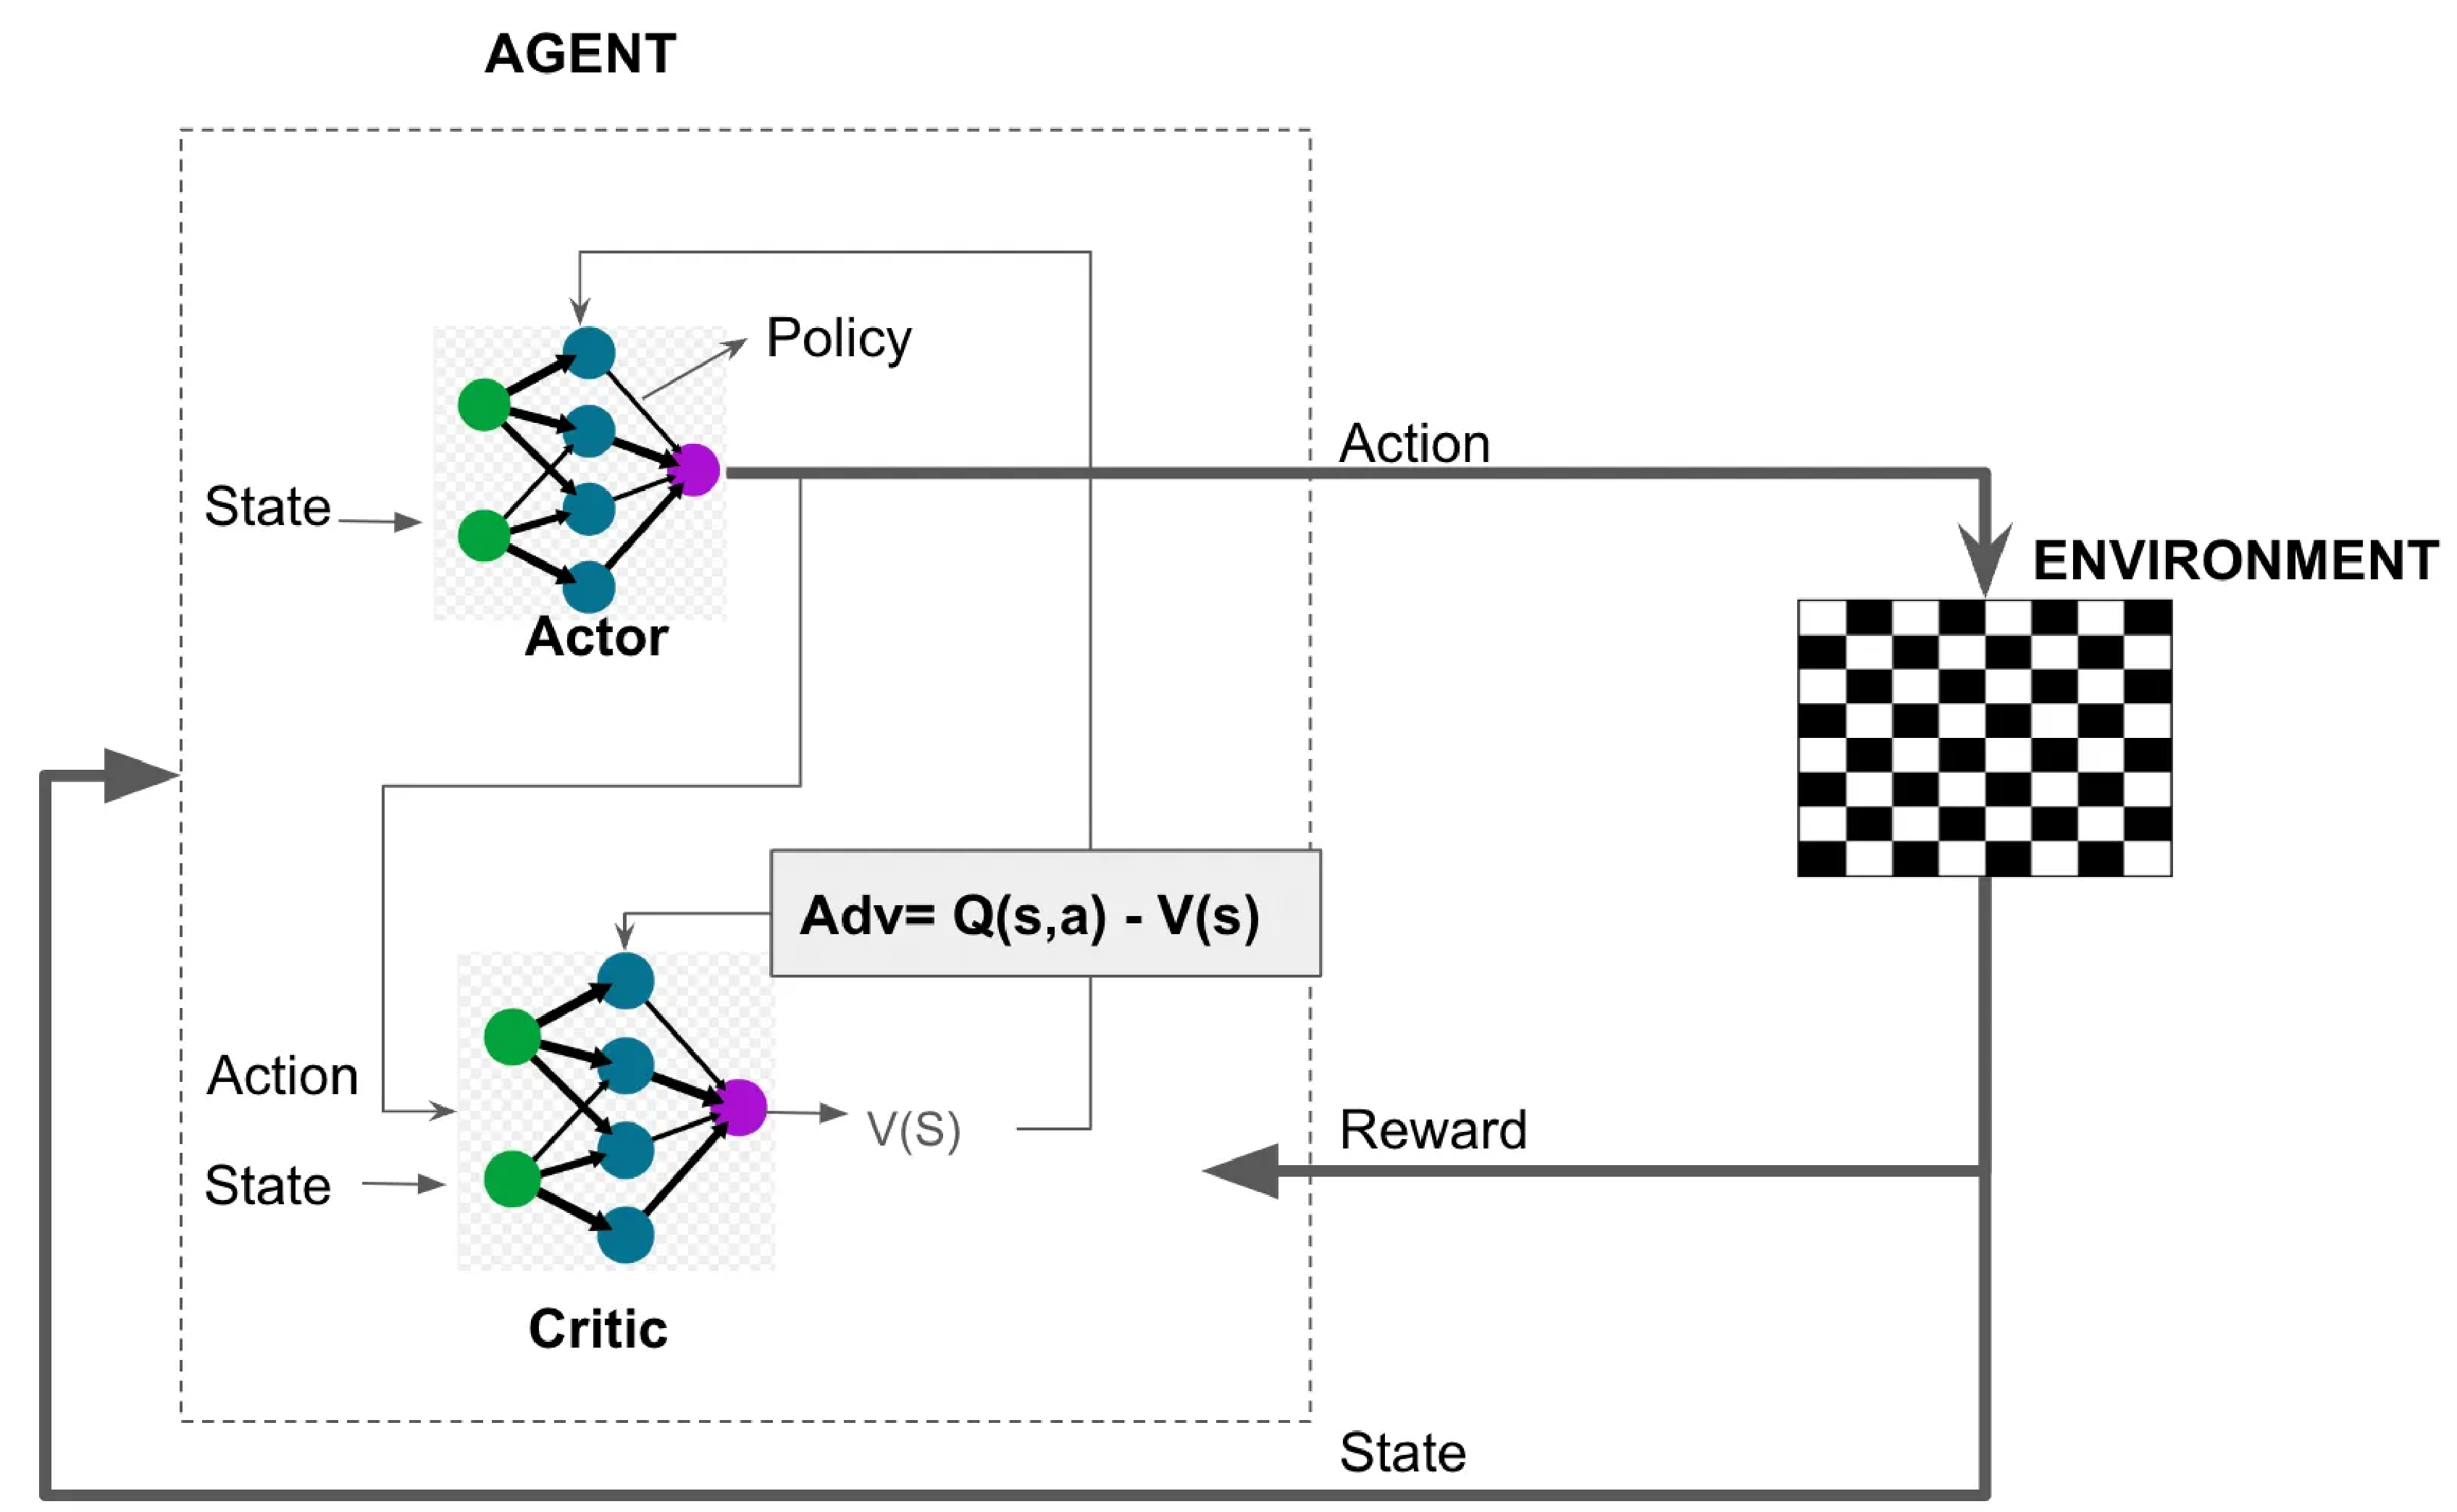
\includegraphics[width=\textwidth]{img/ac_method.pdf}
	\end{column}
\end{columns}
	
\centering

\begin{alertblock}{Learning}
	 	\begin{itemize}
	 		\item The actor outputs the \emph{probability} of taking an \emph{action} in a given \emph{state};
	 		\item The critic estimates the \emph{advantage} of taking that action in that state
	 		\begin{itemize}
				\item $Q(s,a)$ represents the \emph{expected cumulative reward} an agent can expect in a given state;
				\item $V(s)$ represents the \emph{expected future reward} for a given state, \emph{regardless} of the action taken;
			\end{itemize}
	 		\item The advantage function is \emph{backpropagated} to both the networks.
	 	\end{itemize}
\end{alertblock}

\begin{exampleblock}{Advantage function}
	\begin{itemize}
		\item A positive value indicates that  taking that action in that state is expected to yield a better
			outcome than the average action;
		\item Otherwise the agent needs to explore 
			other actions or update the policy to improve the performance.
	\end{itemize}
\end{exampleblock}

\end{frame}
%/////////

%/////////
\begin{frame}{Pseudocode}
%/////////
\begin{figure}
	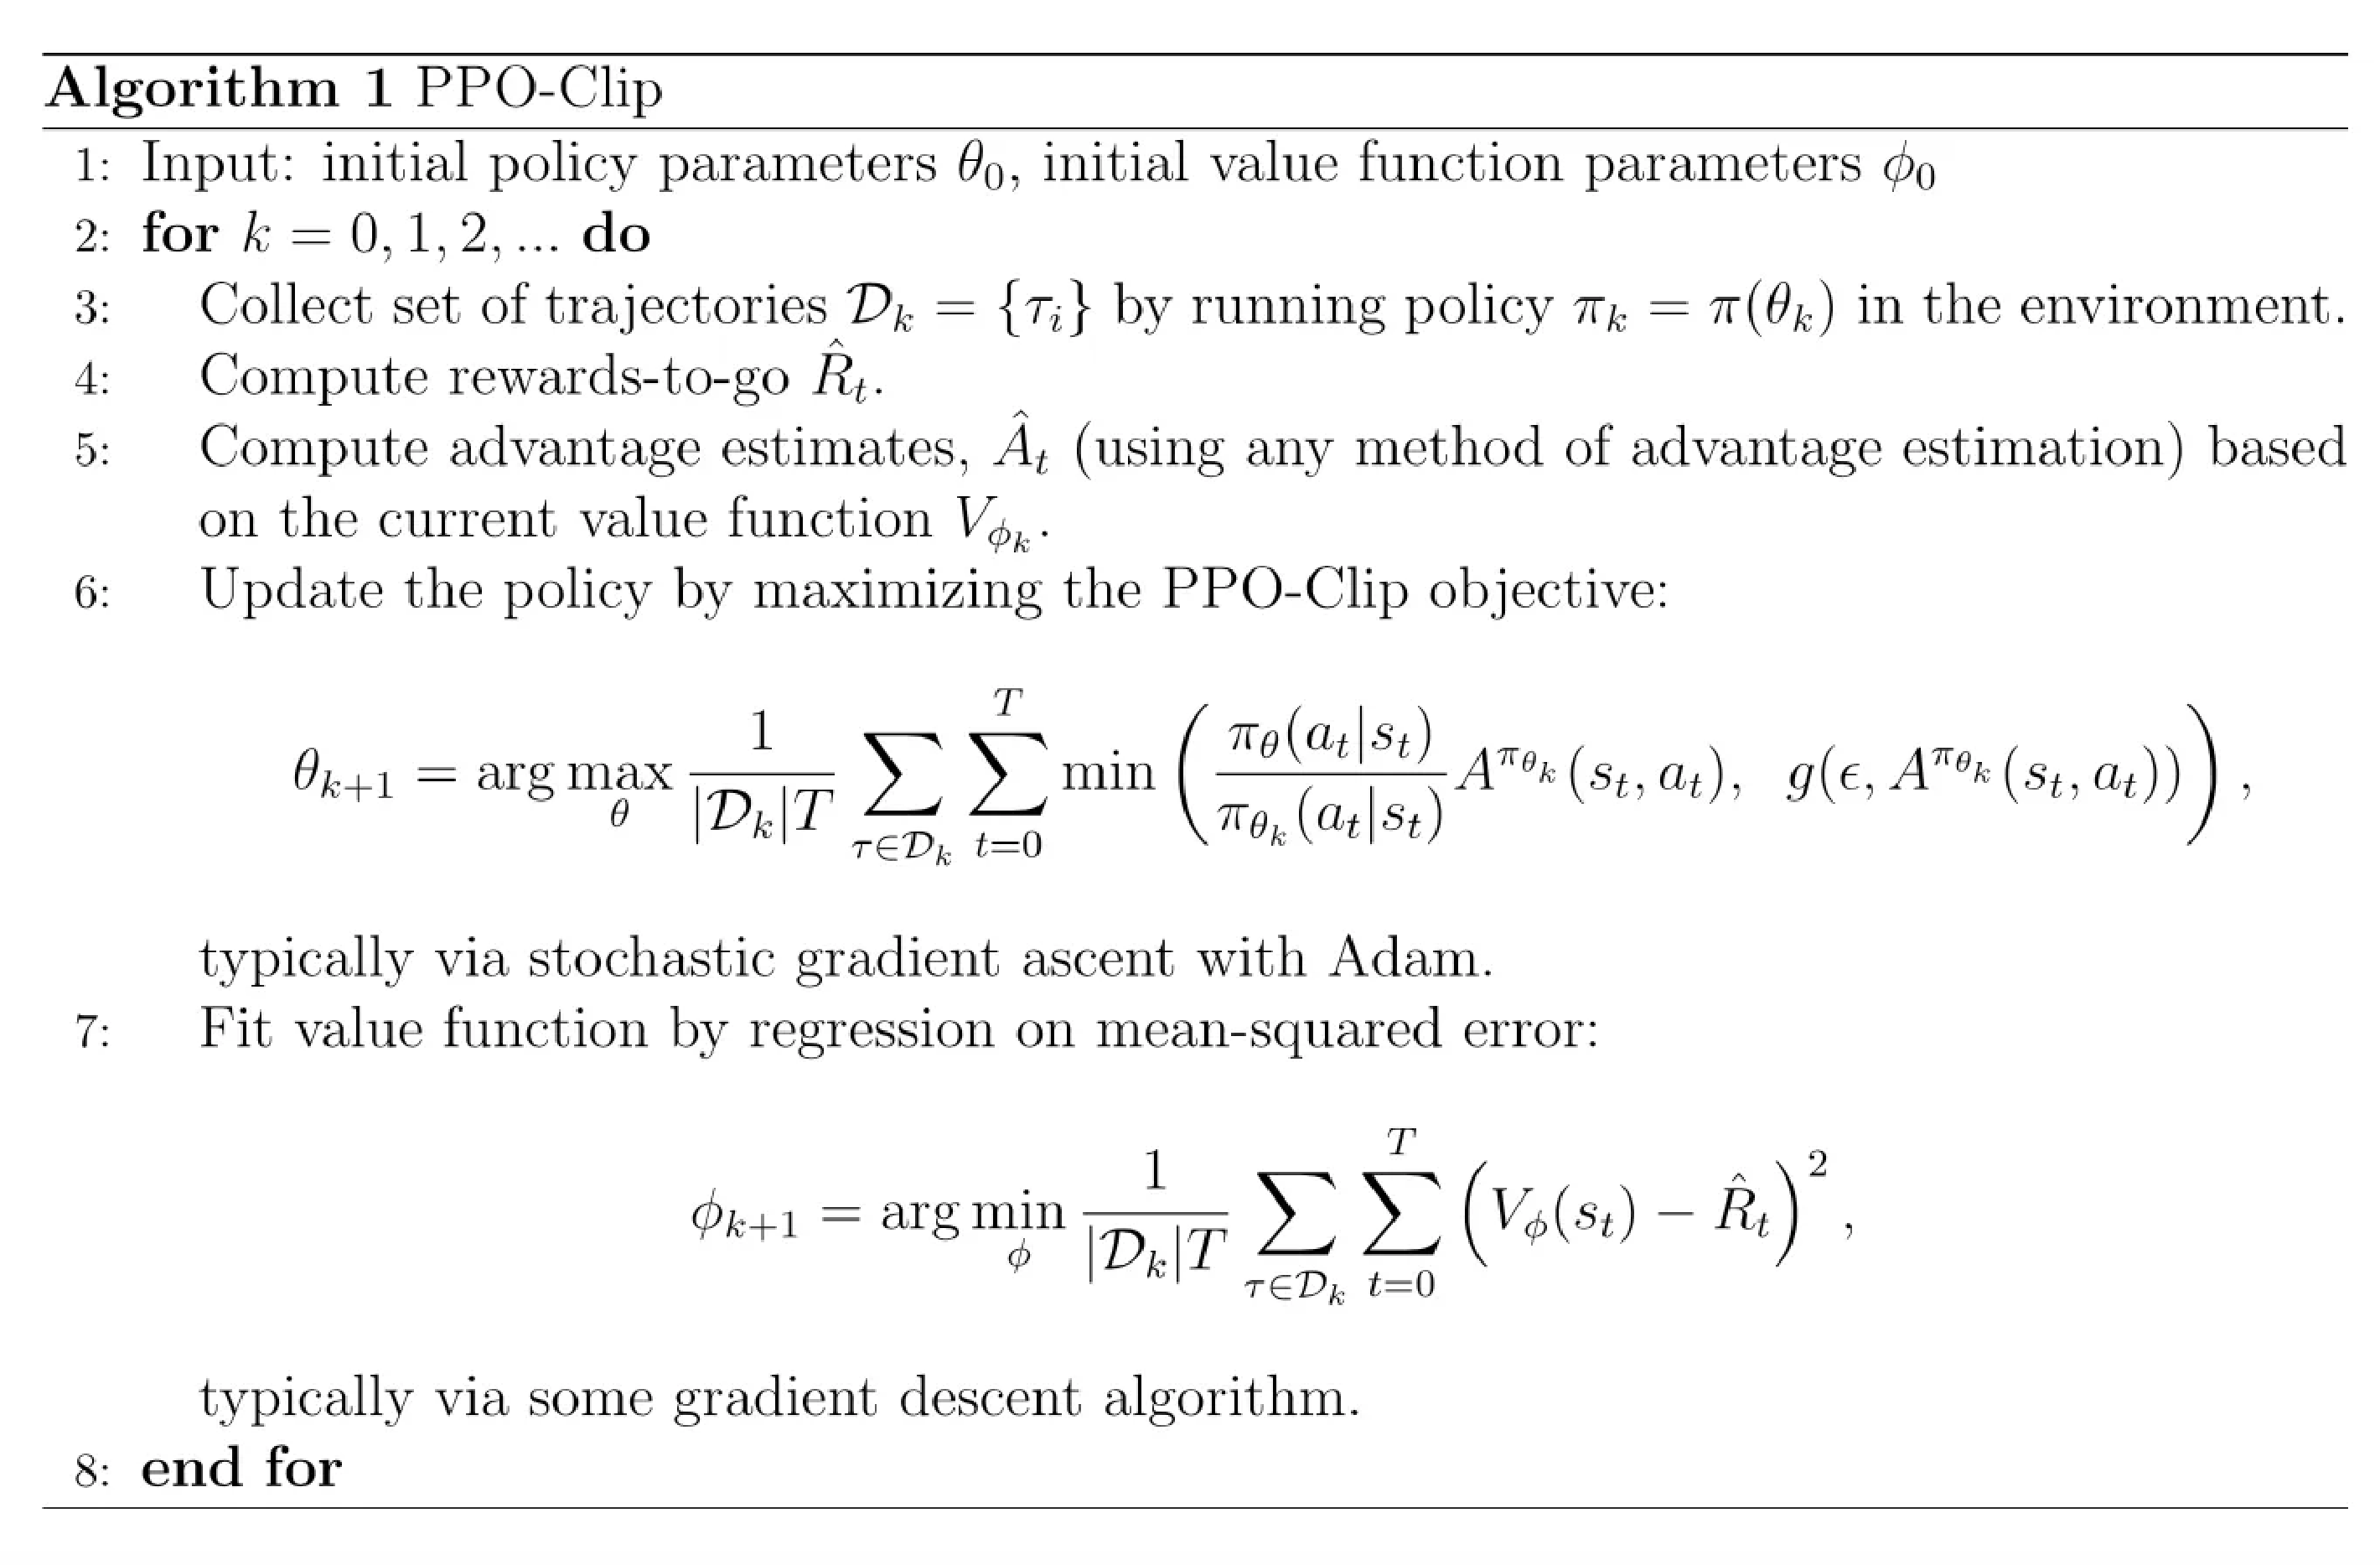
\includegraphics[width=0.9\textwidth]{img/PPO-pseudocode.pdf}
\end{figure}
\end{frame}
%/////////

%/////////
\begin{frame}{Reward to go}
%/////////

\begin{block}{Reward to go}
	The \emph{reward to go} estimates the discounted future reward that can be obtained 
		starting from a given state $S_k$.
\end{block}

\begin{figure}
	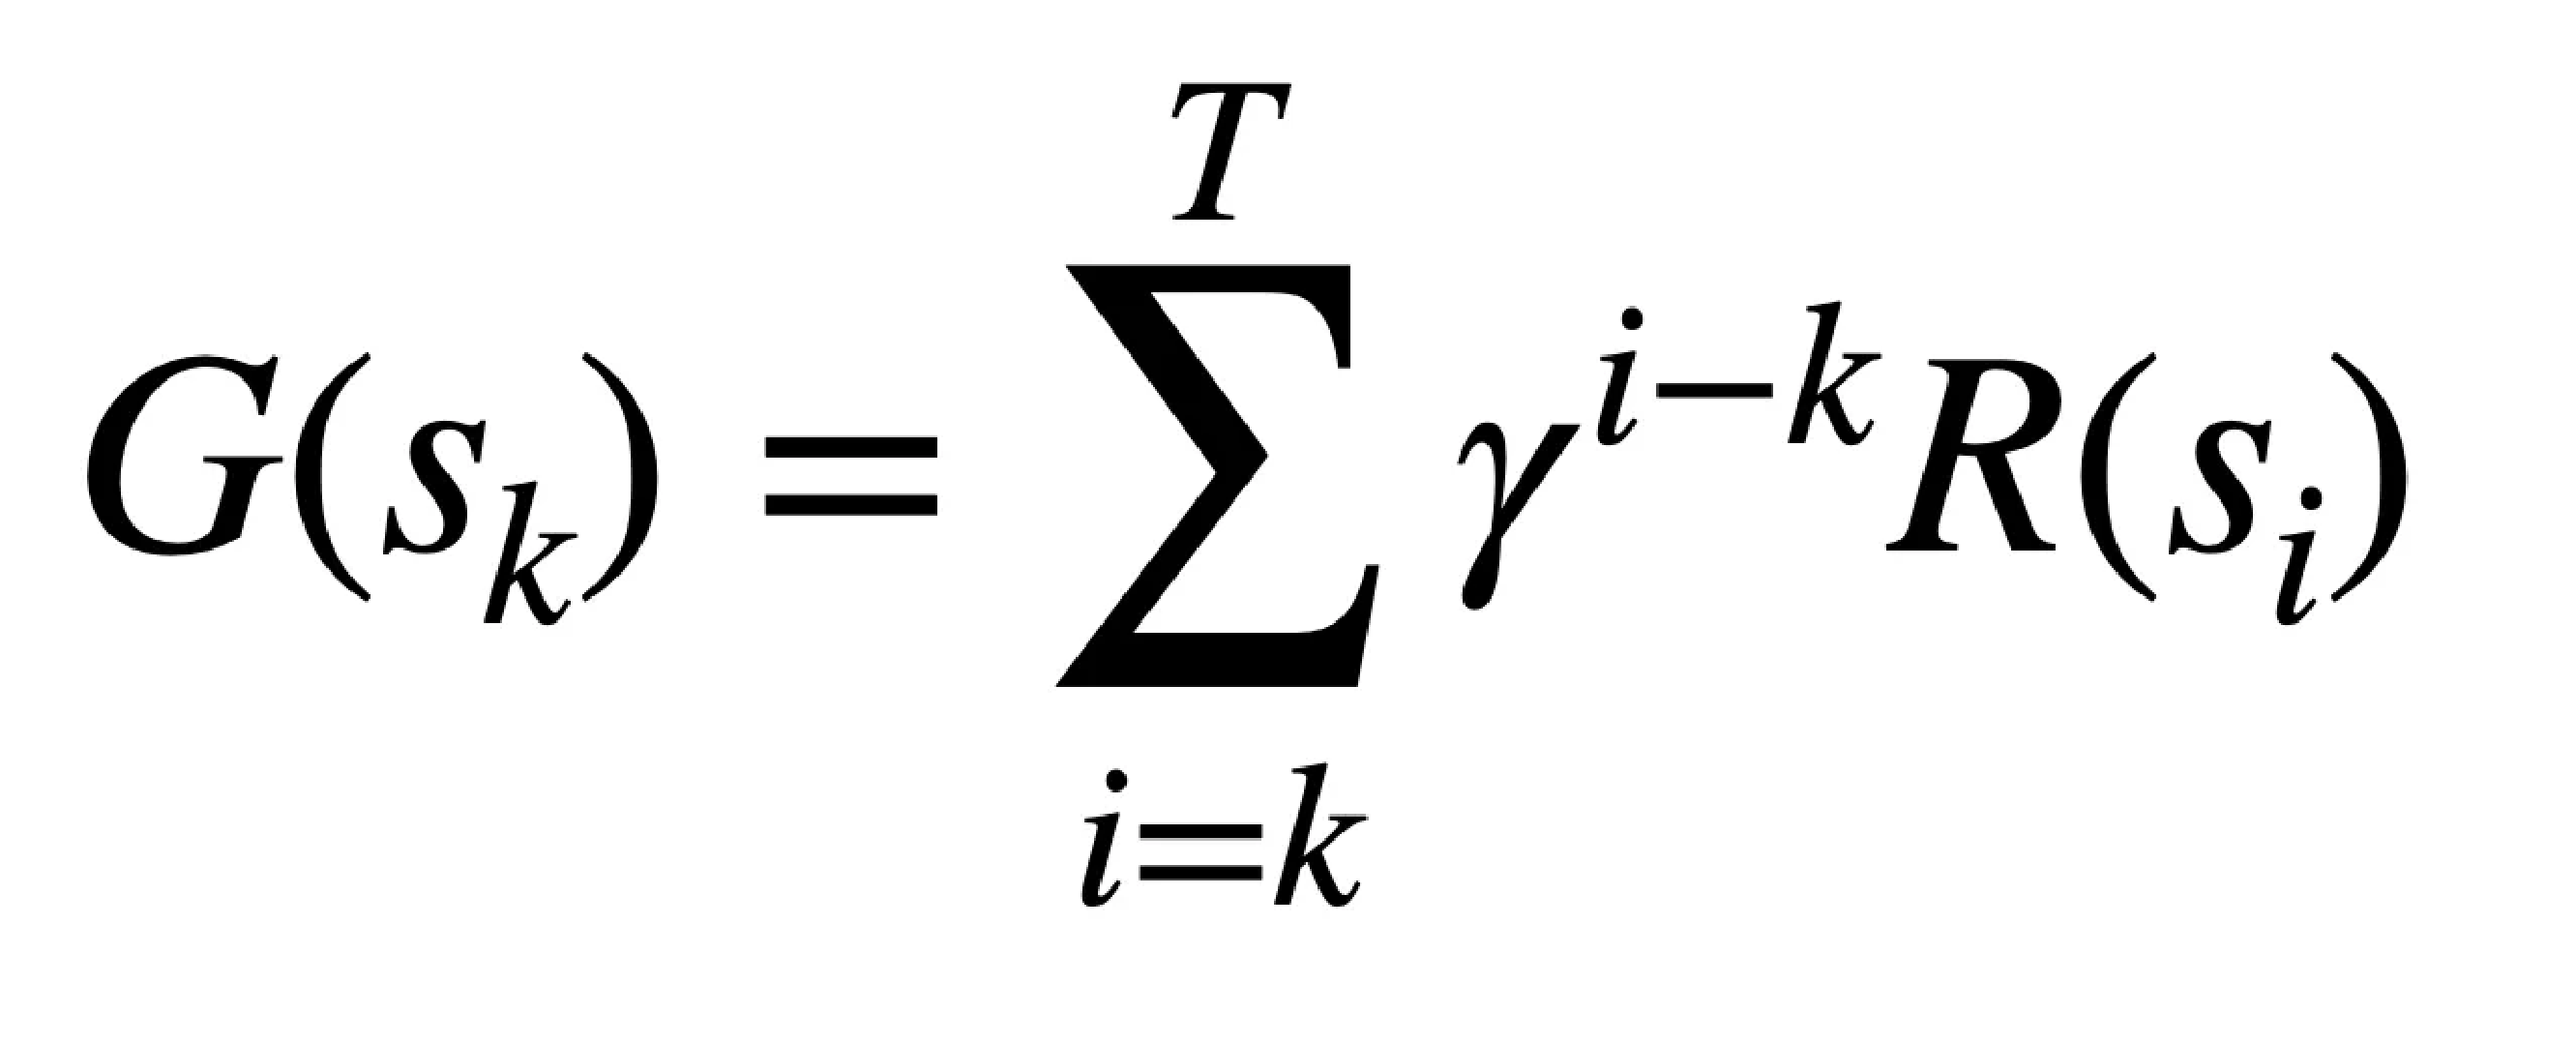
\includegraphics[width=0.6\textwidth]{img/reward-to-go.pdf}
\end{figure}	
\end{frame}
%/////////

%/////////
\begin{frame}{Clipped Loss Function}
%/////////
	
	
\end{frame}
%/////////


%===============================================================================
\section{Project}
%===============================================================================

%/////////
\begin{frame}{Tools}
%/////////
\begin{block}{Tools}
	\begin{itemize}
		\item \textbf{PyTorch}
		\item \textbf{OpenAI Gym}
		\item \textbf{TensorBoard}
		\item \textbf{OpenCV}
		\item \textbf{Numpy}
	\end{itemize}
\end{block}
\end{frame}
%/////////

%/////////
\begin{frame}{Test Environment}
%/////////

% descrivi openai gym
% descrivi l'env scelto

\end{frame}
%/////////

%/////////
\begin{frame}{Implementation}
%/////////

% descrivi la classe PPO
% esempio di codice di come runnare l'esperimento

\end{frame}
%/////////

%/////////
\begin{frame}[fragile]{Normalization}
%/////////
\begin{block}{Advantages Normalization}
	\begin{itemize}
		\item Using raw advantges makes training higly \emph{unstable};
		\item Numerical algorithms behave poorly when \emph{different dimensions} 
			are also \emph{different in scale};
		\item \emph{Normalization} is not in the pseudocode but \emph{in practice} it is very important.
	\end{itemize}
\end{block}

\begin{lstlisting}
A_k = (A_k - A_k.mean()) / (A_k.std() + 1e-10)
\end{lstlisting}

\end{frame}
%/////////


%===============================================================================
\section*{}
%===============================================================================

%/////////
\frame{\titlepage}
%/////////

%===============================================================================
\section*{\refname}
%===============================================================================

%%%%
\setbeamertemplate{page number in head/foot}{}
% %/////////
% \begin{frame}[c,noframenumbering, allowframebreaks]{\refname}
% %\begin{frame}[t,allowframebreaks,noframenumbering]{\refname}
% 	\tiny
% 	\nocite{*}
% 	\printbibliography
% \end{frame}
% %/////////

%%%%%%%%%%%%%%%%%%%%%%%%%%%%%%%%%%%%%%%%%%%%%%%%%%%%%%%%%%%%%%%%%%%%%%%%%%%%%%%%
\end{document}
%%%%%%%%%%%%%%%%%%%%%%%%%%%%%%%%%%%%%%%%%%%%%%%%%%%%%%%%%%%%%%%%%%%%%%%%%%%%%%%%
